%
\documentclass[12pt]{article}

% The usual packages
\usepackage{fullpage}
\usepackage{breakcites}
\usepackage{setspace}
\usepackage{endnotes}
\usepackage{float}
\usepackage{amsmath}
\usepackage{amsfonts}
\usepackage{amssymb}
\usepackage{rotating}
\usepackage{dcolumn}
\usepackage{longtable}
\usepackage{microtype}
\usepackage{graphicx}
\usepackage{hyperref}
%\usepackage[usenames,dvipsnames]{color}
\usepackage{url}
\usepackage{natbib}
\usepackage{framed}
\usepackage{lipsum}
\usepackage[font=small,labelfont=sc]{caption}
\restylefloat{table}
\bibpunct{(}{)}{;}{a}{}{,}

% Set paragraph spacing the way I like
\parskip=0pt
\parindent=20pt

% Define mathematical results
\newtheorem{lemma}{Lemma}
\newtheorem{proposition}{Proposition}
\newtheorem{theorem}{Theorem}
\newtheorem{claim}{Claim}
\newenvironment{proof}[1][Proof]{\begin{trivlist}
\item[\hskip \labelsep {\bfseries #1}]}{\end{trivlist}}
\newenvironment{definition}[1][Definition]{\begin{trivlist}
\item[\hskip \labelsep {\bfseries #1}]}{\end{trivlist}}
\newenvironment{example}[1][Example]{\begin{trivlist}
\item[\hskip \labelsep {\bfseries #1}]}{\end{trivlist}}
\newenvironment{remark}[1][Remark]{\begin{trivlist}
\item[\hskip \labelsep {\bfseries #1}]}{\end{trivlist}}

% Set up fonts the way I like
\usepackage{tgpagella}
\usepackage[T1]{fontenc}
\usepackage[bitstream-charter]{mathdesign}

%% Set up lists the way I like
%Redefine the first level
\renewcommand{\theenumi}{\arabic{enumi}.}
\renewcommand{\labelenumi}{\theenumi}
%Redefine the second level
\renewcommand{\theenumii}{\alph{enumii}.}
\renewcommand{\labelenumii}{\theenumii}
%Redefine the third level
\renewcommand{\theenumiii}{\roman{enumiii}.}
\renewcommand{\labelenumiii}{\theenumiii}
%Redefine the fourth level
\renewcommand{\theenumiv}{\Alph{enumiv}.}
\renewcommand{\labelenumiv}{\theenumiv}

% Create footnote command so that my name
% has an asterisk rather than a one.
\long\def\symbolfootnote[#1]#2{\begingroup%
\def\thefootnote{\fnsymbol{footnote}}\footnote[#1]{#2}\endgroup}

\hypersetup{
 pdftitle={Meaningful Inferences}, % title
 pdfauthor={Kelly McCaskey and Carlisle Rainey}, % author
 pdfkeywords={hypothesis testing} {confidence intervals} {substantive significance}
 pdfnewwindow=true, % links in new window
 colorlinks=true, % false: boxed links; true: colored links
 linkcolor=red, % color of internal links
 citecolor=red, % color of links to bibliography
 filecolor=red, % color of file links
 urlcolor=red % color of external links
}

% enable comments in pdf
\newcommand{\comment}[1]{\textcolor{red}{#1}}

\begin{document}

\begin{center}
{\LARGE Meaningful Inferences}\\\vspace{2mm}
{\large The Key to Substantive Significance is Estimation, Not Hypothesis Tests\symbolfootnote[1]{We thank [many people]. The analyses presented here were conducted with \texttt{R} 3.1.0 and Stata 13. All data and computer code necessary for replication are available at [GitHub Repositroy].}}\\\vspace{2mm}


\vspace{10mm}

Kelly McCaskey\symbolfootnote[2]{Kelly McCaskey is a Ph.D. student in the Department of Political Science, University at Buffalo, SUNY, 520 Park Hall, Buffalo, NY 14260 (\href{mailto:kellymcc@buffalo.edu}{kellymcc@buffalo.edu}).}

\vspace{3mm}

Carlisle Rainey\symbolfootnote[3]{Carlisle Rainey is Assistant Professor of Political Science, University at Buffalo, SUNY, 520 Park Hall, Buffalo, NY 14260 (\href{mailto:rcrainey@buffalo.edu}{rcrainey@buffalo.edu}).}
\end{center}

% Remove page number from first page
%\thispagestyle{empty}

\vspace{10mm}


% Abstract
{\centerline{\textbf{Abstract}}}
\begin{quote}\noindent [Abstract here.] \end{quote}
\thispagestyle{empty}

%\end{document} % uncomment to make a title-page with author info

\newpage
\doublespace
% Set first page of text as page 1. I don't care for this
%   feature because then the page numbers don't correspond
%   to the pdf pages.
%\setcounter{page}{1}

\section*{Introduction}

[introduction here.]

\section*{What We Want To Know}

Most empirical research in political science focuses on estimating the effect $\Delta$ of an explanatory variable $x$ on the expected value of an outcome of interest $y$. Formally, we might suppose that $E(y | x) = f(x)$ and define the ``effect'' or ``quantity of interest'' $\Delta$ as the difference between the average outcomes when $x$ takes on a substantively meaningful high value and low value, so that $\Delta = E(y | x = x_{hi}) - E(y | x = x_{lo}) = f(x_{hi}) - f(x_{lo})$. Importantly, empirical work usually focuses on answering three fundamental questions about the nature of the relationship between $x$ and $y$. Each of these question requires increasing levels of analysis and substantive interpretation and each receives decreasing levels of attention in political science research.

\subsection*{Establish the Sign}

The first question that question that empirical research usually attempts to answer is the direction of the effect. Is the effect positive or negative? Some research argues theoretically and empirically for ``no effect'' or ``a negligible effect'' (e.g., Kam and Palmer 2008, see Rainey 2014), but most hypotheses posit the direction of an effect. \comment{[We could put one or two nice examples here.]} Suppose, for clarity, that the researcher offers a directional research hypothesis, suggesting that an effect of interest $\Delta$ is positive. Formally, we might denote this hypothesis as $H_r: \Delta > 0$. Then the researcher compares this research hypothesis to a null hypothesis that suggests that the research hypothesis is false, or equivalently, that the effect lies outside the region suggested by the research hypothesis. Formally, we might write this as $H_0: \Delta \leq 0$. To assess the evidence against the null hypothesis, the researcher usually calculates a $p$-value, which is the probability of obtaining (hypothetical) data at least as extreme as the observed data if the null hypothesis were true. If this $p$-value is sufficiently small (by convention, less than 0.05), then the researcher rejects the null hypothesis in favor of the research hypothesis. In our example, the researcher would reject negative effects and conclude that the effect is positive. However, if the $p$-value is not sufficiently small, the the researcher declares that the data do not offer compelling evidence against the null and notes that the direction of the effect remains uncertain (though some research incorrectly takes a $p$-value greater than 0.05 as evidence \textit{in favor of} the null hypothesis, see Rainey (2014)).

\comment{[We should discuss that some research focuses exclusively on this ``sign-and-significance'' approach.]}

There are three aspects of this first empirical argument to make note of. First, this style of argumentation is ubiquitous in political science. It is extremely rare to find empirical research in political science that does not perform a hypothesis test of some sort. Second, note that this approach is compelling not because it argues that the observed data are consistent with the researcher's claim, but because the data are inconsistent with other claims. Third, notice that this argument for the direction of the effect explicitly takes into account the uncertainty of the estimated effect. If the uncertainty is large relative to the magnitude of the estimate then the researcher cannot (and usually does not) make confident claims about the direction of the effect of interest. \comment{[We could put a really nice example here of a researcher drawing a cautious conclusion from an insignificant effect.]} However, if the uncertainty is small relative to the size of the estimated effect, then the researcher can draw confident conclusions about the direction of the effect. \comment{[We could put a really nice example here of a researcher drawing a confidence conclusion from a significant effect.]}

\subsection*{Establish the Magnitude}

Yet recent methodological wwork emphasizes that empirical work should go beyond estimating the direction of effects (King, Tomz, Wittenberg 2000; Hanmer and Kalkan 2014; Gross 2014). In addition to the direction of an effect, its size, or magnitude, matters as well. 

Some statistical models have parameters that a naturally interpretable. For example a simple difference-in-means or normal-linear model have directly interpretable coefficients as long as the scales of the variables are reasonable and the model doesn't include non-linear or product terms. Outside of this atypical case, however, the researcher must do additional work to estimate a substantively meaningful quantity of interest.

In discussing how scholars might interpret a model of the effects of education on income, King, Tomz, and Wittenberg (2000, p. 348) write:

\begin{quote}
Bad interpretations are substantively ambiguous and filled with methodological jargon: `the coefficient on education was statistically significant at the 0.05 level.' Descriptions like this are very common in social science, but students, public officials, and scholars should not need to understand phrases like `coefficient,' `statistically significant,' and `the 0.05 level' to learn from the research. Moreover, even statistically savvy readers should complain that the sentences does not convey the key quantity of interest: how much higher the starting salary would be if the student attended college for an extra year.
\end{quote}

The emphasis on effect magnitude is not a new idea. Commenting on the consequences of Fisher's null hypothesis significance test, Yates (1951) writes: ``[I]t has caused scientific workers to pay undue attention to the results of the tests of significance they perform on their data, particularly data derived from experiments, and too little to the estimates of the magnitude of the effects they are investigating.'' Yates continues: ``Tests of significance are preliminary or ancillary. The emphasis on tests of significance, and the consideration of the results of each experiment in isolation, have had the unfortunate consequence that scientific works have regarded the execution of a test of significance on an experiment as the ultimate objective. Results are significant or not significant and that is the end of it.''

Fortunately, with the recent conceptual work by King (1989); Long (1997); King, Tomz, and Wittenberg (2000); Berry, DeMeritt, and Esarey (2010); and Hanmer and Kalkan (2013), political scientists are moving beyond a simple ``sign-and-significance'' approach to presenting substantively meaningful measures of effect magnitude in addition to making compelling arguments about the direction of effect with hypothesis tests. \comment{[We should add a few examples of scholars providing their readers with substantively meaningful measures of effect size, such as first-differences.]}

\subsection*{Establish the Substantive Importance}

But ultimately, researchers want to move beyond the simple presentation of effect magnitude and make a judgment about the meaningfulness of the effects. Are the effects large or small? Are they substantively important? Are they relevant for policy? Are they scientifically important? Hanmer and Kalkan (2013, p. 264) write: ``[W]e take it as given that understanding whether the relationship is substantively significant, rather than just statistically significant, is the ultimate goal, as it is a necessary part of vaulting one's theory.''


\section*{Potential Pitfalls in Reasoning About Effect Magnitude}

There are two possible errors that researchers might make when making claims about the substantive magnitude of the effect. The first has been discussed often and will come as no surprise to some readers. The second is more subtle but has negative consequences that are nearly as severe as the first. The first potential mistake that researchers might make is interpreting the p-value as a measure of magnitude and the second is interpreting the magnitude without explicitly accounting for the uncertainty of the estimate. 

\subsection*{Small $p$-Values Do Not Indicate Large Effect}


A p-value is simply the probability of observing data at least as extreme as the observed data if the null hypothesis were true. All else equal, the p-value usually gets smaller as the effect size under investigation increases. But the $p$-value is also a function of the sample size, for example. ``Very significant'' results (e.g., $p < 0.001$) might simply mean that the research has a large sample. Even if the researcher finds statistically significant results with a small sample, the small $p$-value only indicates that the effect size is large relative to the uncertainty. It says nothing about the size of the estimate relative to some standard of substantive importance. With a very small p-value (e.g., $p < 0.001$), substantive experts might judge the effect to be large, moderate, small, or even negligible. Experts might call some of these effect important, somewhat important, slightly important, or not at all important. The $p$-value is indirectly related to substantive significance at best. This disconnect occurs for two reasons. First, the $p$-value is only partly determined by the effect size--sample size plays a large part as well. Second, the absolute magnitude of the effect cannot be deemed substantively large, small, or negligible without the judgment of a substantive expert. 

\subsection*{Current Practice Does Not Account for Uncertainty}

The standard scientific practice in political science computes substantively interpretable estimates of effects and (1) determines whether these estimates are statistically significant and, if so, (2) makes a judgement about whether the magnitude is substantively important. \comment{[I need to add a cite here, but perhaps several examples will do.]} This two step procedure has three unfortunate consequences.

\begin{enumerate}
\item This tempts political scientists to treat all results that are not statistically significant similarly, drawing no distinction between large, imprecise estimates and small, precise estimates (see Rainey 2014).
\item This tempts political scientists to treat all statistically significant and substantively large estimates similarly, drawing no distinction between large, imprecise estimates and large, precise estimates.
\item This tempts political scientists to treat ``barely significant,'' large estimates and ``almost significant,'' large estimates quite differently, drawing a strong distinction between two similar estimates with similar uncertainty.
\end{enumerate}

\begin{figure}[h]
\begin{center}
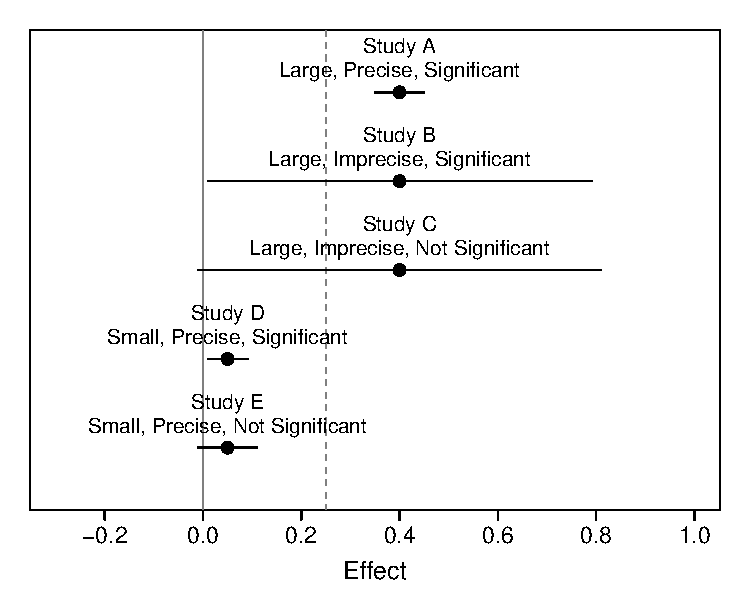
\includegraphics[scale = .6]{figs/example-cis.pdf}
\caption{\comment{[Add caption here.]}}\label{fig:logit}
\end{center}
\end{figure}

\renewcommand{\arraystretch}{1.5}
\begin{table}
\begin{center}
\begin{scriptsize}
\begin{tabular}{|>{\centering\arraybackslash}m{.5in}m{1.75in}>{\centering\arraybackslash}m{1.75in}>{\centering\arraybackslash}
m{1.75in}|}
\hline

Study & Sign and Significance Method & Sign, Significance, Magnitude, and Importance Method & Intuitive Interpretation\\ 
\hline
Study A & ``positive and significant'' & ``positive, significant, and substantively large'' & ``We have strong evidence for a large, substantively meaningful effect.''\\
Study B & ``positive and significant'' & ``positive, significant, and substantively large'' & ``We have only weak evidence for a large, substantively meaningful effect, because the data are also consistent with negligible effects near zero.''\\
Study C & ``not statistically significant'' & ``not statistically significant'' & ``We have only weak evidence for a large, substantively meaningful effect, because the data are also consistent with negligible effects near zero.''\\
Study D & ``positive and significant'' & ``positive and significant, but substantively small' & ``We have strong evidence against a substantively meaningful effect.''\\
Study E & ``not statistically significant'' & ``not statistically significant'' & ``We have strong evidence against a substantively meaningful effect.''\\
\hline
\end{tabular}\caption{\comment{[Add caption here]}}\label{tab:lit}
\end{scriptsize}
\end{center}
\end{table}

The key takeaway point is that it is importance to apply similar standards of evidence to arguments for positive (or negative) effects and arguments for meaningfully positive (or meaningfully negative) effects. The usual logic of hypothesis testing requires that the researcher only declare that an effect is positive if and only if the evidence points overwhelming against negative effects. Similarly, researchers should not declare a positive estimate substantively meaningful simply because it is inconsistent with with negative effects and above some threshold. A better standard of evidence would require that researchers declare an effect meaningful if and only if it is inconsistent with negligible effects.


%\singlespace 
%\normalsize
%\singlespace
%\bibliographystyle{apsr_fs}
%\bibliography{bibliography}

\end{document}

